

\tikzset{every picture/.style={line width=0.75pt}} %set default line width to 0.75pt        

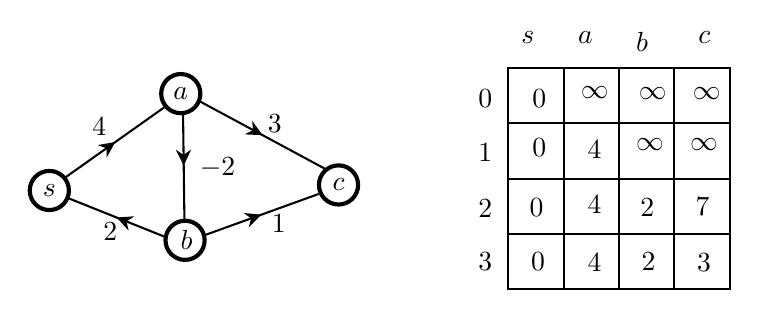
\begin{tikzpicture}[x=0.5pt,y=0.5pt,yscale=-1,xscale=1]
%uncomment if require: \path (0,223); %set diagram left start at 0, and has height of 223

%Shape: Grid [id:dp8546141469296037] 
\draw  [draw opacity=0] (364,36) -- (524,36) -- (524,196) -- (364,196) -- cycle ; \draw   (404,36) -- (404,196)(444,36) -- (444,196)(484,36) -- (484,196) ; \draw   (364,76) -- (524,76)(364,116) -- (524,116)(364,156) -- (524,156) ; \draw   (364,36) -- (524,36) -- (524,196) -- (364,196) -- cycle ;
%Straight Lines [id:da47377092575328894] 
\draw [color={rgb, 255:red, 0; green, 0; blue, 0 }  ,draw opacity=1 ][line width=0.75]    (44,115) -- (116,64) ;
\draw [shift={(80,89.5)}, rotate = 504.69] [fill={rgb, 255:red, 0; green, 0; blue, 0 }  ,fill opacity=1 ][line width=0.08]  [draw opacity=0] (11.61,-5.58) -- (0,0) -- (11.61,5.58) -- (7.71,0) -- cycle    ;
%Straight Lines [id:da6214062451740884] 
\draw [color={rgb, 255:red, 0; green, 0; blue, 0 }  ,draw opacity=1 ][line width=0.75]    (46,130) -- (116,158) ;
\draw [shift={(81,144)}, rotate = 21.8] [fill={rgb, 255:red, 0; green, 0; blue, 0 }  ,fill opacity=1 ][line width=0.08]  [draw opacity=0] (11.61,-5.58) -- (0,0) -- (11.61,5.58) -- (7.71,0) -- cycle    ;
%Straight Lines [id:da8467518623200763] 
\draw [color={rgb, 255:red, 0; green, 0; blue, 0 }  ,draw opacity=1 ][line width=0.75]    (227,127) -- (144,157) ;
\draw [shift={(185.5,142)}, rotate = 160.13] [fill={rgb, 255:red, 0; green, 0; blue, 0 }  ,fill opacity=1 ][line width=0.08]  [draw opacity=0] (11.61,-5.58) -- (0,0) -- (11.61,5.58) -- (7.71,0) -- cycle    ;
%Straight Lines [id:da524270381396472] 
\draw [color={rgb, 255:red, 0; green, 0; blue, 0 }  ,draw opacity=1 ][line width=0.75]    (232,109) -- (141,60) ;
\draw [shift={(186.5,84.5)}, rotate = 208.3] [fill={rgb, 255:red, 0; green, 0; blue, 0 }  ,fill opacity=1 ][line width=0.08]  [draw opacity=0] (11.61,-5.58) -- (0,0) -- (11.61,5.58) -- (7.71,0) -- cycle    ;
%Straight Lines [id:da24886819030904006] 
\draw [color={rgb, 255:red, 0; green, 0; blue, 0 }  ,draw opacity=1 ][line width=0.75]    (129,68) -- (130,145) ;
\draw [shift={(129.5,106.5)}, rotate = 269.26] [fill={rgb, 255:red, 0; green, 0; blue, 0 }  ,fill opacity=1 ][line width=0.08]  [draw opacity=0] (11.61,-5.58) -- (0,0) -- (11.61,5.58) -- (7.71,0) -- cycle    ;

% Text Node
\draw (379.24,49.06) node [anchor=north west][inner sep=0.75pt]   [align=left] {$\displaystyle 0$};
% Text Node
\draw (340.24,88.56) node [anchor=north west][inner sep=0.75pt]   [align=left] {$\displaystyle 1$};
% Text Node
\draw (340.24,129.06) node [anchor=north west][inner sep=0.75pt]   [align=left] {$\displaystyle 2$};
% Text Node
\draw (371.24,7.56) node [anchor=north west][inner sep=0.75pt]   [align=left] {$\displaystyle s$};
% Text Node
\draw (412.24,7.56) node [anchor=north west][inner sep=0.75pt]   [align=left] {$\displaystyle a$};
% Text Node
\draw (454.24,7.56) node [anchor=north west][inner sep=0.75pt]   [align=left] {$\displaystyle b$};
% Text Node
\draw (499.24,7.56) node [anchor=north west][inner sep=0.75pt]   [align=left] {$\displaystyle c$};
% Text Node
\draw (414.24,47.06) node [anchor=north west][inner sep=0.75pt]   [align=left] {$\displaystyle \infty $};
% Text Node
\draw (456.24,48.06) node [anchor=north west][inner sep=0.75pt]   [align=left] {$\displaystyle \infty $};
% Text Node
\draw (495.24,48.06) node [anchor=north west][inner sep=0.75pt]   [align=left] {$\displaystyle \infty $};
% Text Node
\draw (340.24,49.06) node [anchor=north west][inner sep=0.75pt]   [align=left] {$\displaystyle 0$};
% Text Node
\draw (340.24,167.06) node [anchor=north west][inner sep=0.75pt]   [align=left] {$\displaystyle 3$};
% Text Node
\draw (493.24,85.06) node [anchor=north west][inner sep=0.75pt]   [align=left] {$\displaystyle \infty $};
% Text Node
\draw (454.24,85.06) node [anchor=north west][inner sep=0.75pt]   [align=left] {$\displaystyle \infty $};
% Text Node
\draw (379.24,85.06) node [anchor=north west][inner sep=0.75pt]   [align=left] {$\displaystyle 0$};
% Text Node
\draw (419.24,86.06) node [anchor=north west][inner sep=0.75pt]   [align=left] {$\displaystyle 4$};
% Text Node
\draw (419.24,126.06) node [anchor=north west][inner sep=0.75pt]   [align=left] {$\displaystyle 4$};
% Text Node
\draw (419.24,168.06) node [anchor=north west][inner sep=0.75pt]   [align=left] {$\displaystyle 4$};
% Text Node
\draw (377.24,128.06) node [anchor=north west][inner sep=0.75pt]   [align=left] {$\displaystyle 0$};
% Text Node
\draw (378.24,167.06) node [anchor=north west][inner sep=0.75pt]   [align=left] {$\displaystyle 0$};
% Text Node
\draw (457.24,128.06) node [anchor=north west][inner sep=0.75pt]   [align=left] {$\displaystyle 2$};
% Text Node
\draw (458.24,167.06) node [anchor=north west][inner sep=0.75pt]   [align=left] {$\displaystyle 2$};
% Text Node
\draw (498.24,168.06) node [anchor=north west][inner sep=0.75pt]   [align=left] {$\displaystyle 3$};
% Text Node
\draw (497.24,127.06) node [anchor=north west][inner sep=0.75pt]   [align=left] {$\displaystyle 7$};
% Text Node
\draw (69.24,145.53) node [anchor=north west][inner sep=0.75pt]   [align=left] {$\displaystyle 2$};
% Text Node
\draw  [line width=1.5]   (32.38, 124.47) circle [x radius= 14.15, y radius= 14.15]   ;
\draw (32.38,124.47) node   [align=left] {$\displaystyle s$};
% Text Node
\draw  [line width=1.5]   (127.38, 54.47) circle [x radius= 14.15, y radius= 14.15]   ;
\draw (127.38,54.47) node   [align=left] {$\displaystyle a$};
% Text Node
\draw  [line width=1.5]   (130.48, 160.47) circle [x radius= 14.15, y radius= 14.15]   ;
\draw (124.98,160.47) node [anchor=west] [inner sep=0.75pt]   [align=left] {$\displaystyle b$};
% Text Node
\draw  [line width=1.5]   (241.38, 120.47) circle [x radius= 14.15, y radius= 14.15]   ;
\draw (241.38,120.47) node   [align=left] {$\displaystyle c$};
% Text Node
\draw (61.24,69.53) node [anchor=north west][inner sep=0.75pt]   [align=left] {$\displaystyle 4$};
% Text Node
\draw (188,67.47) node [anchor=north west][inner sep=0.75pt]   [align=left] {$\displaystyle 3$};
% Text Node
\draw (191,139.47) node [anchor=north west][inner sep=0.75pt]   [align=left] {$\displaystyle 1$};
% Text Node
\draw (139,98.47) node [anchor=north west][inner sep=0.75pt]   [align=left] {$\displaystyle -2$};


\end{tikzpicture}

